\section{Present your updated concept.}
\label{s_9}

\subsection{What is your design challenge and the respective HMW (how might we) 
question?}
\paragraph{Design Challenge: } 
Refinement of terms and conditions in order to make them easier to read and more 
appealing to the users.
\paragraph{HMW Questions: }
How might we make terms and conditions more legible for the casual users?

\subsection{Describe the idea and the impact it will have on the Challenge you 
have chosen (500 words or less).}

The basic idea is to create a service that will help identify the key parts of 
any online terms and agreements document. This service is based on the open 
source idea, both in development and maintenance. It uses a distributed database 
that contains keywords and key phrases, which is constantly updated, each time 
new laws, regulations, terms and agreements appear. This service will take the 
form of a web browser extension that upon request uses a web crawler will scan 
the document and match each recognised word or phrase retrieved from plain text 
with the ones in the database. Should any matches arise, they will be 
highlighted on the document. For the maintenance and update of this service, a 
user community is responsible. Every user of the service can also be a member of 
the community and can also provide comments on law sections or alterations and 
redefinitions on parts of the document. Every submitted comment by the community, 
will be displayed alongside the highlighted words and phrases in a pop up box 
when the user hovers or clicks each respective item.

The main purpose of this challenge is to find ways to have more transparency on 
where our data is going on the internet. By developing this service, we enable 
users to have a better understanding of the rights they give to each service to 
handle their personal information. That way, before agreeing to use an online 
service, they will be able to know whether their data will stay private, used 
for external purposes or forwarded to third party services. To conclude, users 
can make their own decisions regarding their data, focusing on their privacy and 
not blindly agree to confusing terms because they purposely concealed their 
motives.

\subsection{Present your Storyboard.}

You can find our updated storyboard in the following link: 
\url{https://drive.google.com/open?id=1QnhbVuVnWkFZ8fuaYfQHeT_zflJqK_QtUoV57u9pI0k}.

\subsection{Present your concept in any other format, such as user experience 
diagram, mock-ups, flow charts, etc..}

The mock-up below shows the updated version that takes into consideration the 
feedback of the users.
 
\begin{figure}[H]
\centering
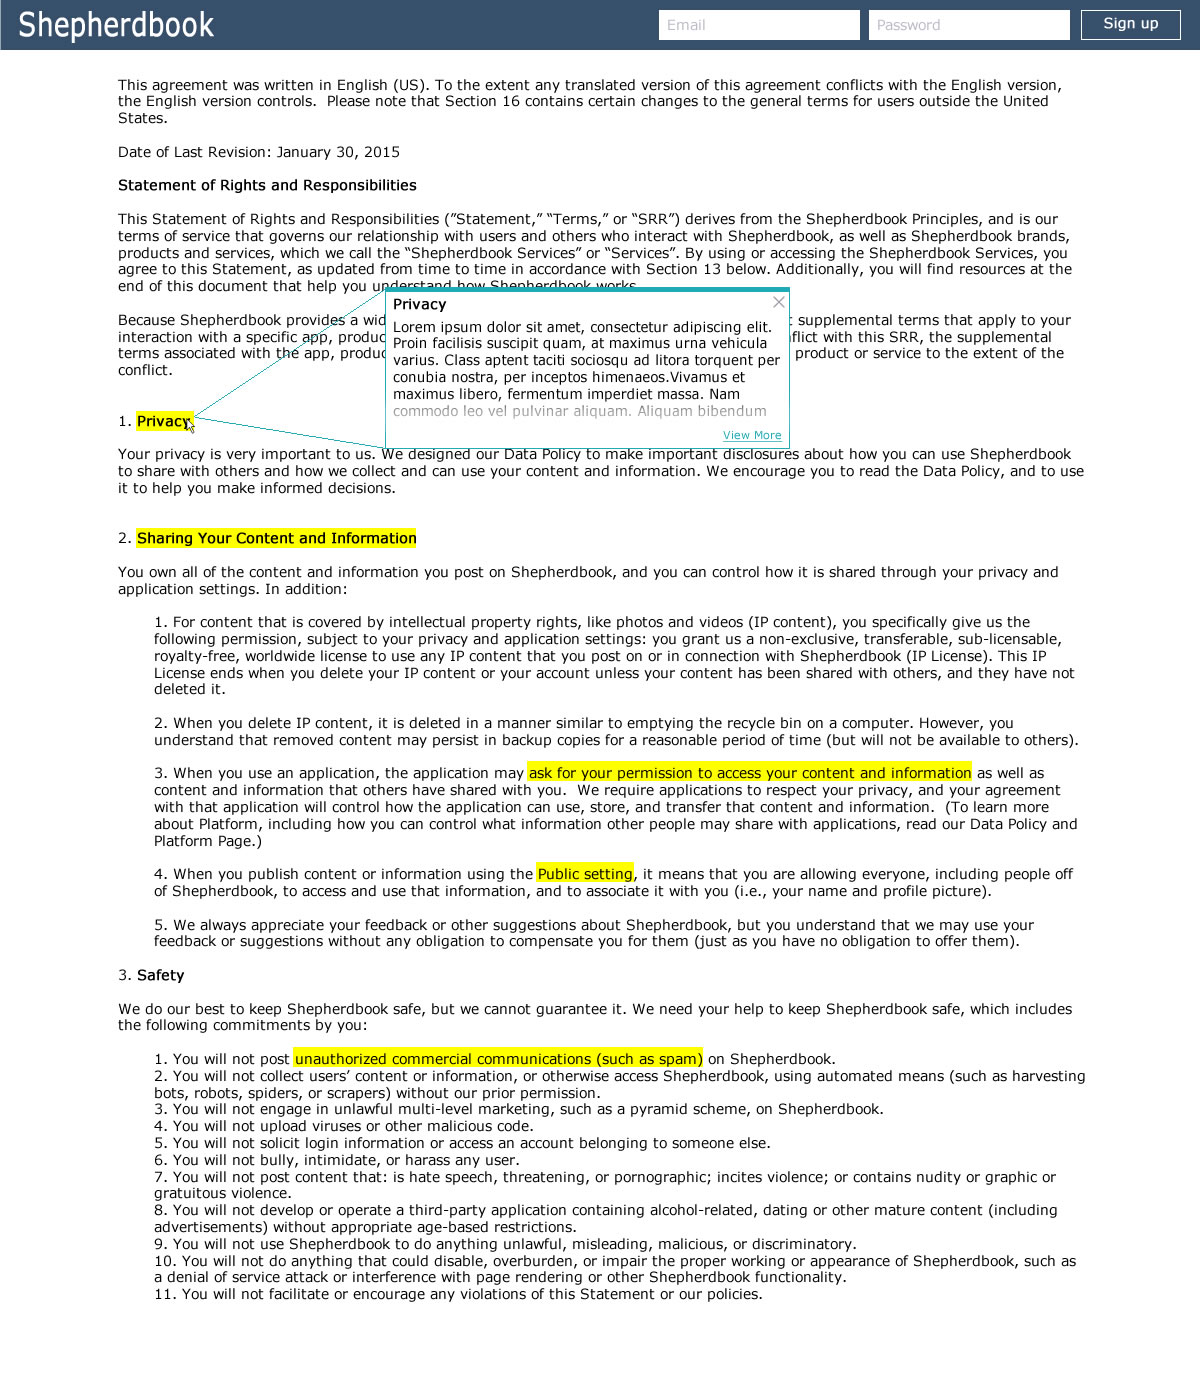
\includegraphics[width=1\columnwidth]{3_HighghtedTerms_Hover_Refined}
\caption{In the updated version, only one comment per highlighted text is shown.}
\end{figure}

